\chapter{Business Forecasting for Valuation}\label{ch:forecast}

\emph{Based on Lecture 03 (file L02, 42 slides): ``Business Forecasting for Valuation''. Session 4 of Part One (workflow step: story $\to$ coherent forecasts). Running case: JJ Jones (value drivers $\to$ forecast statements).}

\section{Where We Are in the Valuation Workflow}

Equity story $\to$ Financial statements $\to$ \textbf{Forecasts} $\to$ Cash flows $\to$ Discount rate $\to$ Terminal value $\to$ Multiples $\to$ Value bridge $\to$ Recommendation.

\begin{keybox}[Today]
\textbf{Equity story + financial statements $\longrightarrow$ coherent forecasts $\longrightarrow$ projected cash flows}
\end{keybox}

\textbf{Today's professional task.} You receive a management business plan. Your job is \textbf{not} to copy it into Excel; it is to \textbf{assess whether it is coherent enough to value}:
\begin{itemize}
  \item identify the business story;
  \item translate the story into value drivers;
  \item build integrated forecast statements;
  \item test whether sales, margins, CapEx, working capital and financing assumptions fit together;
  \item understand how JJ Jones' value drivers generate projected statements.
\end{itemize}

\textbf{Plan for today.}
\begin{center}
\small
\begin{tabularx}{\textwidth}{@{}lXX@{}}
\toprule
\textbf{Layer} & \textbf{What we learn} & \textbf{Why it matters}\\
\midrule
CORE & Equity story $\to$ value drivers $\to$ forecast statements & JJ Jones, project\\
CORE & Projecting IS, BS, and CF statements & Integrated valuation model\\
PRO & Market analysis, strategy, actions, assumptions & Professional business planning\\
TECH & Model architecture, cash sweep, circularity & Avoid spreadsheet/model errors\\
RESEARCH PREVIEW & Forecast coherence & Bridge to special topic\\
PRACTICE & JJ Jones & Turn assumptions into statements\\
\bottomrule
\end{tabularx}
\end{center}

% =====================================================================
\section{From Equity Story to Value Drivers}

\subsection{Overview I: The Phases of Business Planning}

Business planning consists of several interrelated phases:
\begin{center}
\begin{tikzpicture}[
  num/.style={fill=navy,text=white,font=\bfseries,minimum width=0.9cm,minimum height=0.95cm},
  txt/.style={draw=gray!60,fill=gray!6,rounded corners=2pt,text width=10cm,minimum height=0.95cm,align=left,font=\small,inner sep=5pt}]
\foreach \i/\t in {1/{Thorough analysis of company features, market(s), positioning and past performance},
                   2/{Definition of precise competitive strategies},
                   3/{Definition of actions needed to pursue these strategies},
                   4/{Definition of quantitative assumptions underpinning forecast financial statements},
                   5/{Preparation of forecast financial statements}}{
  \node[num] (n\i) at (0,-1.15*\i) {\i};
  \node[txt,anchor=west] at (0.6,-1.15*\i) {\t};
}
\end{tikzpicture}
\end{center}

\subsection{Overview II: Numbers Without Narrative}

There are at least \textbf{three significant dangers} when numbers are used without any narrative in constructing valuations:
\begin{center}
\begin{tikzpicture}[b/.style={fill=navy,text=white,rounded corners=3pt,minimum width=3cm,minimum height=1.1cm,align=center,font=\bfseries}]
\node[b] (a) at (0,0) {Plug-\&-point\\exercise};
\node[b] (b) at (4,0) {Spreadsheet\\Nirvana};
\node[b] (c) at (8,0) {No logical tie\\breaker};
\draw[-{Stealth},line width=3pt,navy!30] (a)--(b); \draw[-{Stealth},line width=3pt,navy!30] (b)--(c);
\end{tikzpicture}
\end{center}
In a good valuation, \textbf{numbers are bound together coherently and story-telling is kept grounded with numbers}:
\begin{itemize}
  \item develop a narrative for the business you are valuing or considering investing in;
  \item test the narrative against history, experience and common sense;
  \item convert key parts of the narrative into value drivers;
  \item connect value drivers to a valuation;
  \item keep the feedback loop open.
\end{itemize}
\begin{keybox}[Key message]
A business plan must be both \textbf{narratively credible} and \textbf{financially coherent}.
\end{keybox}
\begin{addbox}
\textbf{Plug-\&-point}: you plug in numbers and point at the output. \textbf{Spreadsheet nirvana}: the model looks precise just because it is detailed. \textbf{No logical tie breaker}: when two analysts disagree, without a story there is no way to decide which number is more reasonable.
\end{addbox}

\subsection[What Is a Coherent Plan?]{What Is a Coherent Plan? \layer{CORE}}

A plan is coherent when:
\begin{enumerate}
  \item the business story explains the value drivers;
  \item value drivers map into financial-statement items;
  \item sales growth is supported by capacity, CapEx, and working capital;
  \item margin improvement has an operational explanation;
  \item financing assumptions are consistent with cash-flow deficits or surpluses;
  \item long-run assumptions are reachable from the explicit forecast period.
\end{enumerate}
\begin{keybox}[Bottom line]
A plan can be \textbf{plausible line by line and still be incoherent as a system}.
\end{keybox}

\textbf{JJ Jones: today's running case.} We will translate a compact set of value drivers into: income-statement forecasts, PPE forecasts, balance-sheet forecasts, free-cash-flow forecasts (Section~\ref{sec:jjjones}).

\subsection[Market Analysis]{Market Analysis \layer{PRO}}

To prepare accurate and coherent forecasts, it is necessary to analyse the markets the firm operates in. The articulation and complexity of the analysis depends on several variables:
\begin{center}
\begin{tikzpicture}[h/.style={fill=navy,text=white,font=\small\bfseries,minimum width=11cm,minimum height=0.55cm},
  d/.style={fill=navy!15,font=\small,minimum width=11cm,minimum height=0.55cm}]
\foreach \i/\a/\b in {0/{Unrelated businesses}/{The firm operates in unrelated businesses (\emph{holding firms})},
                      1/{Different geographical markets}/{The firm operates in different geographical markets (\emph{multinational firms})},
                      2/{Different distribution channels}/{The business units target different distribution channels$^{(1)}$},
                      3/{Residual}/{Hybrid situations that mix the cases above}}{
  \node[h] at (0,-1.9*\i) {\a};
  \node[d] at (0,-1.9*\i-0.55) {\b};
}
\foreach \i in {0,1,2} \draw[-{Stealth},line width=4pt,navy] (0,-1.9*\i-0.9) -- (0,-1.9*\i-1.55);
\end{tikzpicture}
\slidefig{(1) For instance, a firm could sell its products through both its proprietary website and a network of retail stores.}
\end{center}

\subsection[Competitive Strategy]{Competitive Strategy \layer{PRO}}

The competitive strategies should be prepared both at (1) the \textbf{overall company level} and (2) any \textbf{single business-unit level} (if any).
\begin{center}
\begin{tikzpicture}[hd/.style={fill=navy,text=white,font=\small\itshape,minimum width=3.6cm,minimum height=0.55cm},
  it/.style={fill=navy!15,font=\small,minimum width=3.6cm,minimum height=0.5cm}]
\node[draw,dashed,rounded corners,minimum width=9.6cm,minimum height=0.6cm,font=\bfseries] at (2.4,0.7) {Overall competitive strategy};
\node[hd] at (0,0) {Company level}; \node[hd] at (4.8,0) {Business unit level};
\foreach \i/\a/\b in {1/Operating sectors/Geographical markets,2/Legal structure/Competitive positioning,3/Corporate structure/Distribution channel(s),4/Finance structure/Business model,5/Tax planning/Supply chain integration,6/Intangibles/Physical places to occupy}{
  \node[it] at (0,-0.62*\i) {\a}; \node[it] at (4.8,-0.62*\i) {\b};}
\draw[{Stealth}-{Stealth},line width=6pt,gray!40] (1.95,-1.9) -- (2.85,-1.9);
\end{tikzpicture}
\end{center}

\begin{figure}[H]
\centering
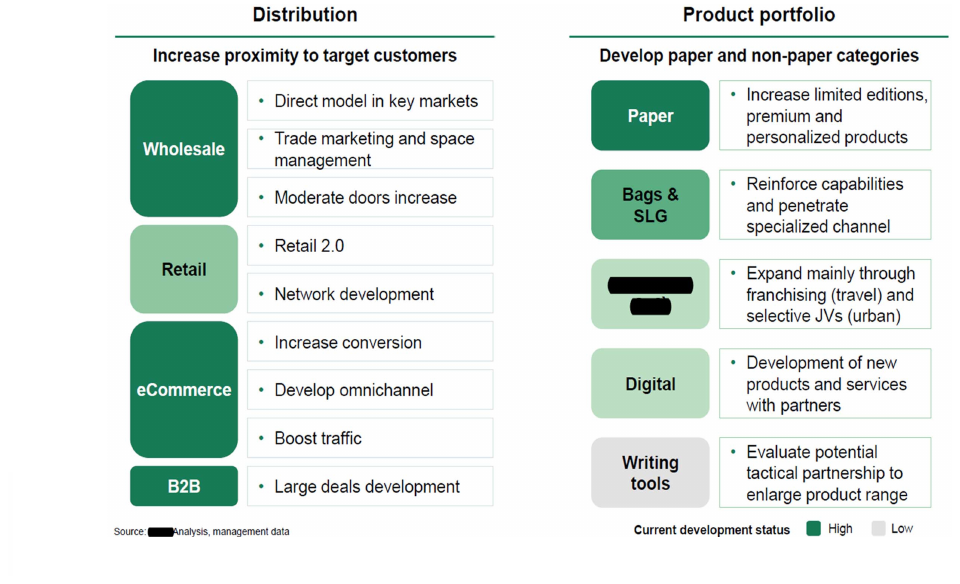
\includegraphics[width=0.85\textwidth]{L02_slide12.png}
\caption{Competitive strategy example (slide screenshot): \textbf{Distribution} -- increase proximity to target customers (Wholesale: direct model in key markets, trade marketing and space management, moderate doors increase; Retail: Retail 2.0, network development; eCommerce: increase conversion, develop omnichannel, boost traffic; B2B: large deals). \textbf{Product portfolio} -- develop paper and non-paper categories (Paper, Bags \& SLG, a redacted category, Digital, Writing tools).}
\end{figure}

\subsection[Action-Taking]{Action-Taking \layer{CORE}}

Once the competitive strategies are defined, the focus is on the \textbf{actions needed to implement them}. Each action should be matched with the following prescriptions:
\begin{center}
\begin{tikzpicture}[a/.style={fill=navy,text=white,minimum width=9cm,minimum height=0.75cm,font=\normalsize,anchor=west}]
\foreach \i/\t in {0/Clear objectives to be pursued,1/Impacts on financial statements,2/Expected realization timing,3/Execution risks and people in charge}{
  \node[a] at (0.6*\i,-0.95*\i) {\hspace{0.8cm}\t};
  \draw[fill=white,draw=navy!40] (0.6*\i,-0.95*\i) circle (0.42);}
\end{tikzpicture}
\end{center}
\slidefig{The credibility of a business plan largely depends on how clearly the mapping of the actions to implement it is set out.}

\begin{figure}[H]
\centering
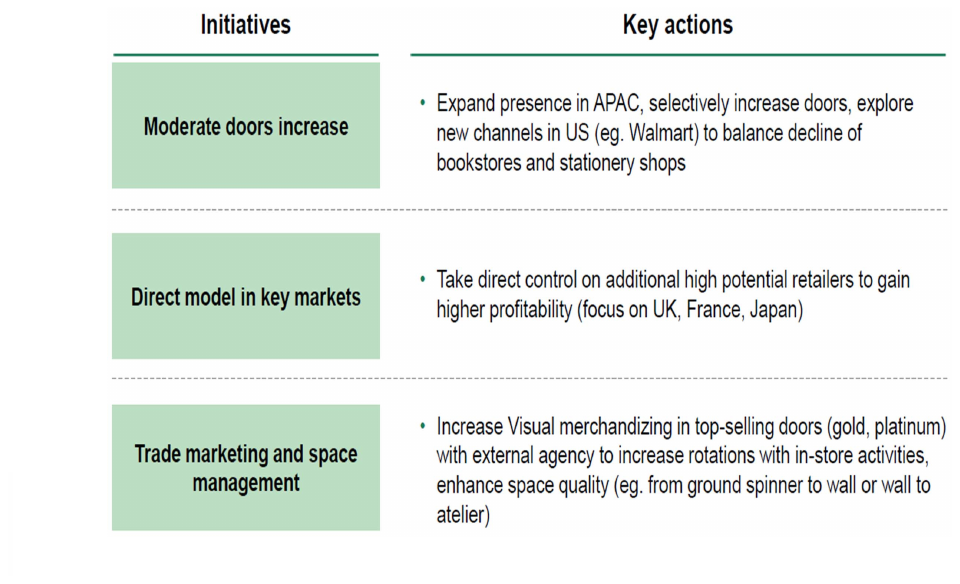
\includegraphics[width=0.72\textwidth]{L02_slide14.png}
\caption{Action-taking example (slide screenshot). \emph{Moderate doors increase}: expand in APAC, selectively increase doors, explore new US channels (e.g., Walmart) to balance the decline of bookstores and stationery shops. \emph{Direct model in key markets}: take direct control of high-potential retailers for higher profitability (UK, France, Japan). \emph{Trade marketing and space management}: visual merchandising in top-selling doors with an external agency, in-store activities, better space quality.}
\end{figure}

\subsection[Quantitative Assumptions]{Quantitative Assumptions \layer{CORE}}

The planning activity ends with a forecast financial statement, based on a series of \textbf{quantitative assumptions}:
\begin{center}
\begin{tabular}{@{}>{\columncolor{navy}\color{white}\bfseries}c p{9cm}@{}}
Macroeconomic & Different for each \emph{geographic area} (GDP, inflation, forex, \dots)\\[3pt]
Business activity & Evolution of \emph{key financials} (sales, costs, working capital, ratios, \dots)\\[3pt]
Corporate structure & Changes at \emph{corporate level} (capital structure, fiscal policy, surplus assets, \dots)
\end{tabular}
\end{center}

\subsection[Revenue Forecast Assumptions]{Revenue Forecast Assumptions \layer{CORE}}

\begin{center}
\begin{tikzpicture}[font=\small,b/.style={draw=navy,minimum width=1.9cm,minimum height=0.55cm,align=center},
  e/.style={-{Stealth[length=1.6mm]},navy}]
\node[b] (rev) at (0,0) {Revenue};
\node[b] (p) at (2.6,1.3) {Price}; \node[b] (v) at (2.6,-1.3) {Volume};
\node[b] (ms) at (5.3,0.2) {Market Size}; \node[b] (sh) at (5.3,-2.6) {Market Share};
\node[b] (g) at (8.0,1.6) {Growth}; \node[b] (t) at (8.0,0.9) {Threats}; \node[b] (o) at (8.0,0.2) {Opportunities};
\node[b] (u) at (8.0,-0.8) {Uniqueness}; \node[b] (aw) at (8.0,-1.5) {Awareness}; \node[b] (lo) at (8.0,-2.2) {Loyalty}; \node[b] (pa) at (8.0,-2.9) {Patents};
\node[b] (ad) at (10.8,0.2) {Advertising}; \node[b] (pr) at (10.8,-0.5) {Promotion}; \node[b] (sf) at (10.8,-1.2) {Sales Force};
\node[b] (dc) at (10.8,-1.95) {Distribution\\[-3pt]Coverage}; \node[b] (av) at (10.8,-2.8) {Availability};
\foreach \x in {p,v} \draw[e] (\x.west) -- (rev.east);
\foreach \x in {ms,sh} \draw[e] (\x.west) -- (v.east);
\foreach \x in {g,t,o} \draw[e] (\x.west) -- (ms.east);
\foreach \x in {u,aw,lo,pa} \draw[e] (\x.west) -- (sh.east);
\foreach \x in {ad,pr,sf,dc,av} \draw[e] (\x.west) -- (u.east);
\end{tikzpicture}
\end{center}
\begin{keybox}[Professional rule]
\textbf{Do not forecast revenue growth as one number unless you can explain the whole logic behind it.}
\[
\text{Revenue} = \text{Price}\times\text{Volume} = \text{Price}\times\text{Market size}\times\text{Market share}
\]
\end{keybox}
\begin{addbox}[Growth decomposition]
$(1+g_{\text{Rev}})=(1+g_{\text{price}})(1+g_{\text{market}})(1+g_{\text{share}})$. Example: price $+2\%$, market $+5\%$, share $+3\%$ $\Rightarrow$ $1.02\times1.05\times1.03-1=10.3\%$.
\end{addbox}

\subsection[Modelling]{Modelling \layer{CORE}}

\begin{center}
\begin{tikzpicture}
\draw[thick,gray!60,fill=navy!5] (-3.2,1.9) -- (3.2,1.9) -- (0.7,-1.3) -- (-0.7,-1.3) -- cycle;
\fill[navy!80] (-1.05,0.85) circle (0.85); \node[text=white,font=\footnotesize\bfseries,align=center] at (-1.05,0.85) {Mkt\\Analysis};
\fill[navy] (1.05,0.85) circle (0.85); \node[text=white,font=\footnotesize\bfseries] at (1.05,0.85) {Strategy};
\fill[navy!55] (0,-0.4) circle (0.75); \node[text=white,font=\footnotesize\bfseries,align=center] at (0,-0.4) {HPs \&\\Actions};
\draw[-{Stealth},line width=6pt,navy!25] (0,-1.35) -- (0,-1.95);
\node[align=center] at (0,-2.4) {\underline{Integrated Forecast Financial Statement}\\{\footnotesize (This is where the equity story becomes numbers)}};
\end{tikzpicture}
\end{center}

% =====================================================================
\section{Building the Integrated Forecast Model}

\subsection[Modelling Basics I--II: The Ten Steps]{Modelling Basics I--II: The Ten Steps \layer{CORE}}

\begin{center}
\begin{tikzpicture}[num/.style={fill=navy,text=white,font=\bfseries,minimum width=0.8cm,minimum height=0.6cm},
  txt/.style={draw=gray!60,fill=gray!6,text width=5.6cm,minimum height=0.6cm,font=\small,inner sep=3pt,anchor=west}]
\foreach \i/\t in {1/Set up the model template,2/Input historical financials,3/Calculate ratios,4/Build assumptions,5/{Project the IS (\underline{leave out interest})}}{
  \node[num] at (0,-0.75*\i) {\i}; \node[txt] at (0.5,-0.75*\i) {\t};}
\foreach \i/\t in {6/{Project the BS (\underline{leave out cash and debt})},7/Project the CF statement,8/Balance the BS,9/{Model interest expense/income},10/{Create summary/output pages}}{
  \node[num] at (7.2,-0.75*\i+3.75) {\i}; \node[txt] at (7.7,-0.75*\i+3.75) {\t};}
\end{tikzpicture}
\end{center}
\begin{addbox}[Why interest, cash and debt come last]
They depend on the financing need, which is only known once operations have been projected. Financing is the last layer and must never ``plug'' operating mistakes.
\end{addbox}

\subsection[Main Aspects and Precautions of Model Set-Up]{Main Aspects and Precautions of Model Set-Up \layer{PRO}}

\textbf{Crucial aspects:}
\begin{enumerate}
  \item One-sheet vs multi-sheet model.
  \item \textbf{Matrix integrity}: a given column refers to a specific year in all sheets.
  \item Key sheets: assumptions/inputs; secondary calculations; debt schedule; income statement; balance sheet; cash-flow statement; summary ratios; output.
\end{enumerate}
\textbf{Precautions:}
\begin{enumerate}
  \item Modelling standards: (a) \textbf{Accurate} -- always proof-read your model (sanity, matrix, and stress check); (b) \textbf{Coherent} -- assumptions about individual items should fit with each other; flexible -- no hard numbers in formulae; user friendly -- break down complex calculations.
  \item Learn keyboard shortcuts (more accurate, more coherent, and more sleep).
  \item Use comments to indicate sources.
  \item Formatting and colour coding: inputs, links to other sheets, and formulae in three different colours (style sheet).
  \item Be able to print your model at any time.
\end{enumerate}

\subsection[Modelling Basics III: Historical Inputs]{Modelling Basics III: Historical Inputs \layer{CORE}}

When collecting historical financial inputs:
\begin{enumerate}
  \item A standard model typically has \textbf{3--5 years} of historical data.
  \item IS and BS line items should reflect the structure of the company's published financials.
  \item Some items must be forecast separately even if not broken down in the financials:
  \begin{itemize}
    \item \textbf{D\&A}: generally included in COGS and SG\&A; find the total in the CF statement;
    \item \textbf{interest expense}: can be expressed net of interest income;
    \item \textbf{interest income}: can be netted from interest expense or included in other income;
    \item \textbf{non-recurring items}: identify them and separate them from the ordinary line items.
  \end{itemize}
  \item Some items may be aggregated for simplicity (other assets/liabilities).
\end{enumerate}

\subsection[Modelling Basics IV: Ratios and Assumptions]{Modelling Basics IV: Ratios and Assumptions \layer{PRO}}

\begin{enumerate}
  \item Identify key ratios to analyse historical performance: IS (growth/margins); BS (days receivable, payable, inventory).
  \item Make assumptions on the evolution of key ratios based on: trends in historical ratios; strategic assessment; market consensus for the company; market consensus for competitors (peer group).
  \item Cross-check the assumptions against: \textbf{historical trends} (any abrupt jumps?); \textbf{internal coherence} (is the evolution of related items coherent?); \textbf{external consistency} (in line with consensus?).
\end{enumerate}

\subsection[Modelling Basics V--VI: Model Architecture]{Modelling Basics V--VI: Model Architecture \layer{TECH}}

\begin{center}
\scriptsize
\begin{tabular}{@{}p{3.7cm}p{4.6cm}p{4.2cm}@{}}
\toprule
\textbf{Income Statement} & \textbf{Retained Earnings} & \textbf{Supporting Schedules}\\
Revenues; Operating expenses; \textbf{EBIT}; Interest expense; EBT; Taxes; \textbf{Net income} &
Beginning balance; + Net income; $-$ Preferred dividends; $-$ Common dividends; = Ending balance &
\emph{Competitive analysis}: general economy, industry, comparables.\newline
\emph{Fixed assets}: capacity needs, fixed-asset requirements, CapEx, depreciation.\\
\midrule
\textbf{Balance Sheet} & \textbf{Free Cash Flows} & \emph{Income taxes}: expense, deferred, NOL carryforward, payable.\\
Operating assets; Fixed assets; \textbf{Total assets}; Operating liabilities; Debt; Total liabilities; Preferred stock; Common stock; Retained earnings; Stockholders' equity; \textbf{Total liabilities + equity} &
EBIT; $-$ Taxes on EBIT; + Non-cash expenses; $-$ $\Delta$Required cash; $-$ $\Delta$Working cap.; $-$ CapEx; = \textbf{Unlevered FCF}; $-$ Interest; + Interest tax shield; $-$ Preferred div.; + $\Delta$Debt; + $\Delta$Preferred; = \textbf{Equity FCF}; $-$ Common div.; = $\Delta$Excess cash; + $\Delta$Required cash; = \textbf{$\Delta$Cash} & \emph{Financing}: debt and interest, preferred stock, common stock.\\
\bottomrule
\end{tabular}
\end{center}

\begin{figure}[H]
\centering
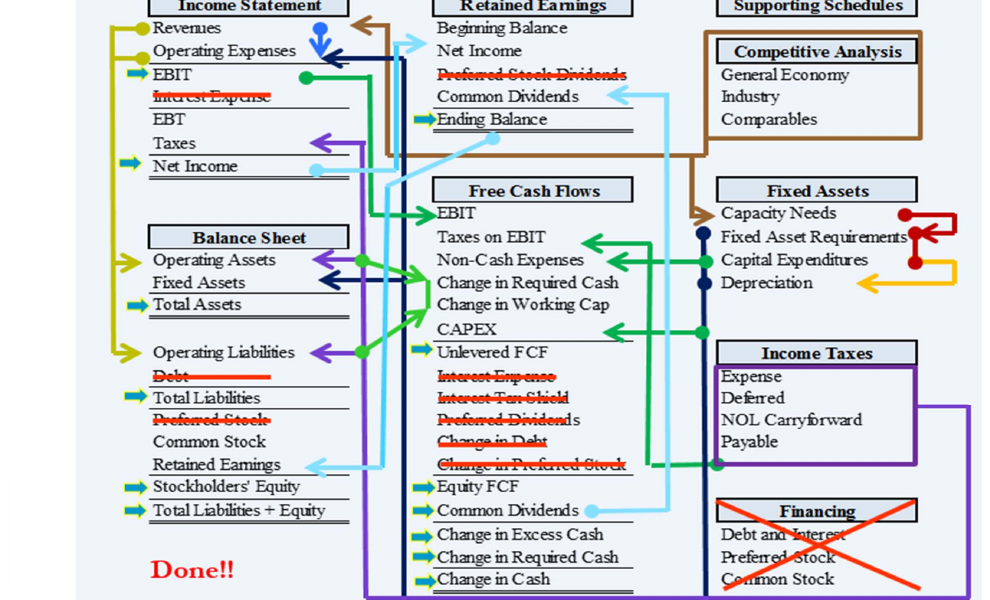
\includegraphics[width=0.85\textwidth]{L02_slide26.png}
\caption{Modelling Basics VI (slide screenshot): how every block of the model links. The financing items (interest expense, debt, preferred stock and dividends, interest tax shield, change in debt and in preferred stock) and the whole Financing schedule are crossed out, and the operating model is ``Done!!''.}
\end{figure}
\begin{addbox}
The message of Modelling Basics VI: the \textbf{operating (unlevered) model} can be completed through the unlevered FCF \textbf{without any financing assumption}. Financing (debt, interest, preferred) is added at the end to balance the BS. This mirrors the split between FCFO (no financing) and FCFE (with financing) in Chapter~\ref{ch:fcf}.
\end{addbox}

\subsection[Projecting the Income Statement]{Projecting the Income Statement \layer{CORE}}

\begin{center}
\begin{tikzpicture}[h/.style={fill=navy,text=white,font=\bfseries,minimum width=7.2cm,minimum height=0.6cm,anchor=north},
  d/.style={fill=navy!15,font=\small,text width=6.9cm,align=center,minimum height=0.6cm,anchor=north,inner sep=3pt}]
\foreach \c/\i/\a/\b in {0/0/{Sales (\emph{forecast growth})}/{Price growth drivers (inflation, strategy); volume growth drivers (tot.\ market \emph{vs} market share)},
                      0/1/{COGS and SG\&A}/{Project COGS and SG\&A as a \% of sales},
                      0/2/{Depreciation}/{Project depreciation as \% of PPE at the \textbf{beginning} of the period},
                      1/0/{Amortization}/{Project amortization based on specific intangible-asset estimation},
                      1/1/{Interest income and expense}/{Leave out until you are done with the rest of the model},
                      1/2/{Taxes}/{Consider effective \emph{vs} marginal tax rate}}{
  \node[h] (h\c\i) at (7.6*\c,-2.95*\i) {\a}; \node[d] (d\c\i) at (h\c\i.south) {\b};}
\foreach \c in {0,1} \foreach \i/\j in {0/1,1/2} \draw[-{Stealth},line width=4pt,navy] ([yshift=-1pt]d\c\i.south) -- ([yshift=1pt]h\c\j.north);
\end{tikzpicture}
\end{center}
\begin{keybox}[Coherence checks]
If revenue grows, do margins, D\&A and capacity assumptions still make sense?\\
If debt, cash, taxes, or interest change, do the projected interest and tax assumptions follow?
\end{keybox}

\textbf{Further issues \layer{PRO}}
\begin{itemize}
  \item \textbf{Net income}: normalize net income for non-recurring items.
  \item \textbf{EPS}: basic \emph{vs} diluted; net income \emph{vs} normalized net income.
  \item \textbf{DPS}: DPS growth rate \emph{vs} payout ratio.
  \item \textbf{Equity}: use net income and dividends to complete the equity base analysis.
\end{itemize}

\subsection[Projecting the Balance Sheet]{Projecting the Balance Sheet \layer{CORE}}

\begin{center}
\small
\begin{tabularx}{\textwidth}{@{}>{\bfseries}p{4.2cm}X@{}}
\toprule
Working capital & Driven by sales and COGS (receivable, inventory and payable days)\\
Fixed assets (PPE schedule in secondary calcs) & CapEx as a fixed component + \% of sales; maintenance \emph{vs} expansion\\
Goodwill & Keep it flat\\
Financial investments \textnormal{(PRO)} & Fair value estimated to stay flat\\
Other operating liabilities \textnormal{(PRO)} & Driven by sales\\
Equity \textnormal{(PRO)} & Take it from the secondary calculation sheet\\
Short and long-term debt \textnormal{(PRO)} & Leave out until you are done with the rest of the model\\
\bottomrule
\end{tabularx}
\end{center}
\begin{keybox}[Coherence checks]
If revenue grows, do receivables, inventories, payables, and PPE grow consistently?\\
Are cash and debt balancing the model, or are they hiding operating-forecast mistakes?
\end{keybox}
\begin{addbox}[Days and ratio formulas used in practice (and in JJ Jones)]
\vspace{-6pt}
\begin{align*}
\text{Receivables} &= \text{Revenue}\times\frac{\text{DSO}}{365} & \text{Inventory} &= \text{COGS}\times\frac{\text{DIO}}{365}\\
\text{Payables} &= \text{COGS}\times\frac{\text{DPO}}{365} & \text{Net PPE} &= \frac{\text{Net PPE}}{\text{Revenue}}\times\text{Revenue}\\
\text{CapEx} &= \Delta\text{Net PPE}+\text{Depreciation}
\end{align*}
\end{addbox}

\subsection[Projecting the Cash-Flow Statement]{Projecting the Cash-Flow Statement \layer{CORE}}

\begin{keybox}[The 100\% rule]
You are \textbf{100\% certain} to be able to obtain the firm's change in cash from the change in all non-cash BS accounts: read that again, you have to be no less than 100\% certain. The CF statement captures the change in every balance-sheet item and yields the resulting change in cash.
\end{keybox}
General rules:
\begin{itemize}
  \item \textbf{Assets up, cash down}; \textbf{liabilities up, cash up};
  \item the change in WC captures changes in operating assets/liabilities;
  \item CapEx and D\&A capture changes in fixed assets;
  \item net income and dividends capture changes in retained earnings.
\end{itemize}

\textbf{Two key cash-flow measures \layer{PRO}}
\begin{center}
\begin{tabular}{@{}rl@{\hspace{1.5cm}}rl@{}}
\multicolumn{2}{@{}l}{\textbf{1. Net cash flow}} & \multicolumn{2}{l}{\textbf{2. Cash available for debt repayment}}\\
$+$ & Operating cash flow & $+$ & Operating cash flow (starting from NI)\\
$+$ & Investing cash flow & $+$ & Investing cash flow\\
$+$ & Financing cash flow & $+$ & Equity issuance\\
\cmidrule{1-2}
$=$ & Net cash flow ($=\Delta$cash) & $-$ & Dividends/stock repurchase\\
\cmidrule{3-4}
&& $=$ & Cash flow available for debt repayment (CFADR)\\
&& $-$ & Cash required (for day-to-day activities)\\
\cmidrule{3-4}
&& $=$ & Cash available for debt repayment (CADR)
\end{tabular}
\end{center}
\begin{keybox}
\begin{gather*}
\text{Beginning cash} + \text{Net cash flow} = \text{Ending cash}\\
\text{Beginning cash} + \text{CFADR} - \text{Cash required} = \text{CADR}
\end{gather*}
\end{keybox}

\subsection[Final Procedures]{Final Procedures \layer{TECH}}

\textbf{I. Balancing the BS.}
\begin{itemize}
  \item Complete the debt schedule.
  \item Use a simple \textbf{cash sweep}: all cash available for debt repayment pays down debt, starting from short-term and moving to long-term debt.
  \begin{itemize}
    \item If CADR is \textbf{positive}, it goes to repay debt.
    \item If CADR is \textbf{negative}, short-term debt is issued to cover the shortage of cash and the minimum level of operating cash required to run operations smoothly.
  \end{itemize}
  \item Link the resulting short-term and long-term debt balances to the BS (in turn reflected in the CF statement), and link the resulting cash balance in the CF statement to the BS.
\end{itemize}

\textbf{II. Circularity.} When interest expense is computed on \textbf{average} debt and interest income on \textbf{average} cash, the model becomes circular:
\begin{center}
\begin{tikzpicture}[c/.style={fill=navy,text=white,rounded corners=3pt,minimum width=2.2cm,minimum height=0.9cm,align=center,font=\small}]
\node[c] (i) at (0,1.5) {Interest\\expenses/income};
\node[c] (n) at (2.6,0) {Net\\income};
\node[c] (c) at (0,-1.5) {Cash flow};
\node[c] (d) at (-2.6,0) {Debt/cash\\ending balance};
\draw[-{Stealth},gray,thick,bend left=25] (i) to (n); \draw[-{Stealth},gray,thick,bend left=25] (n) to (c);
\draw[-{Stealth},gray,thick,bend left=25] (c) to (d); \draw[-{Stealth},gray,thick,bend left=25] (d) to (i);
\end{tikzpicture}
\end{center}
A (less accurate) alternative that does not require iteration is to use the \textbf{opening balance} of debt and cash.

\textbf{III. Summary and output pages} (PRO). Build ratios on projected performance: growth; activity/asset turnover; solvency/credit; profitability; returns. If needed, prepare output sheets that are easy to paste into presentations (a life saver when assumptions change at the last minute, e.g., before a board meeting) and clear when printed from Excel.

% =====================================================================
\section{JJ Jones Case: From Value Drivers to Forecast Statements}\label{sec:jjjones}

\begin{exbox}[JJ Jones: value drivers]
\small
\begin{minipage}[t]{0.48\linewidth}
\textbf{\color{keyred}Income statement}
\begin{itemize}[leftmargin=*]
  \item Revenue growth -- simple 10\% growth
  \item Cost of goods sold -- 60\% of revenues
  \item Operating expenses -- 10\% of revenues
  \item Depreciation -- 10 years
  \item Income tax rate -- 40\% on all income
\end{itemize}
\textbf{\color{keyred}Assets}
\begin{itemize}[leftmargin=*]
  \item Excess assets (cash and other) -- \$0
  \item Required cash balance -- 5\% of revenues
  \item Accounts receivable -- 50 days$^*$
  \item Inventory -- 80 days$^*$
  \item Other current assets -- 6\% of revenues
  \item Net PPE to revenues -- 1.2 ratio$^*$
  \item Other assets -- \$0
\end{itemize}
\end{minipage}\hfill
\begin{minipage}[t]{0.48\linewidth}
\textbf{\color{keyred}Liabilities and preferred stock}
\begin{itemize}[leftmargin=*]
  \item Accounts payable -- 40 days$^*$
  \item Accrued expenses -- 20\% of revenues
  \item Non-current liabilities -- 10\% of revenues
  \item Other income -- \$0 (excess assets related)
  \item Interest rate -- 8\% (beginning balance)
  \item Preferred dividend rate -- 10\% (beginning balance)
  \item Debt -- retire current portion of long-term debt; increase long-term debt if the company has insufficient cash flow (same interest rate)
  \item Preferred stock -- no change
\end{itemize}
\end{minipage}

\smallskip
\footnotesize $^*$ based on ending balance (not average balance)
\end{exbox}

\textbf{Discussion Questions.} Given the value drivers, prepare JJ Jones' (i) income-statement forecasts; (ii) PPE forecasts; (iii) balance-sheet forecasts; (iv) free-cash-flow forecasts.

\textbf{What JJ Jones tests} (slide):
\begin{enumerate}
  \item Can you translate assumptions into forecast statements?
  \item Can you keep the three statements linked?
  \item Can you distinguish required cash from excess cash?
  \item Can you forecast working capital from days ratios?
  \item Can you forecast PPE from the PPE/revenue ratio?
  \item Can you let debt/cash balance the model instead of plugging operations?
  \item Can you compute FCFO and FCFE from the resulting statements?
\end{enumerate}

\begin{addbox}[How each driver becomes a line item]
\begin{itemize}[leftmargin=*]
  \item Revenue$_t$ = 1.10 $\times$ Revenue$_{t-1}$; COGS = 60\%; Opex = 10\%; taxes = 40\% of EBT.
  \item Depreciation = Gross PPE$_{\text{begin}}$ / 10 (10-year straight line).
  \item Net PPE$_t$ = 1.2 $\times$ Revenue$_t$ $\Rightarrow$ CapEx$_t$ = Net PPE$_t$ $-$ Net PPE$_{t-1}$ + Depreciation$_t$.
  \item AR = Rev $\times$ 50/365; Inventory = COGS $\times$ 80/365; AP = COGS $\times$ 40/365 (ending balances).
  \item Interest = 8\% $\times$ beginning debt; preferred dividends = 10\% $\times$ beginning preferred (beginning balances avoid circularity).
  \item Debt is the \textbf{balancing item}: repay the current portion of LTD; if cash flow is insufficient, issue new LTD. Since excess assets $= 0$, any surplus would be paid out (no excess cash accumulates).
\end{itemize}
\end{addbox}

\begin{exbox}[Illustrative one-year forecast (base-year figures assumed by us; the class handout has the real ones)]
\small
\textbf{Assumed base year (Y0):} revenue 1,000; cash 50 (= 5\%); AR $1{,}000\times50/365=136.99$; inventory $600\times80/365=131.51$; other CA 60; gross PPE 2,000, accumulated depreciation 800, net PPE 1,200 (= 1.2 $\times$ revenue); AP $600\times40/365=65.75$; accrued 200; current LTD 50; LTD 500; non-current liabilities 100; preferred 100; common equity (balancing) 562.74.

\medskip
\begin{minipage}[t]{0.47\linewidth}
\textbf{(i) Income statement, Y1}\\[2pt]
\begin{tabular}{@{}lr@{}}
Revenue ($1{,}000\times1.1$) & 1,100.00\\
$-$ COGS (60\%) & (660.00)\\
$-$ Operating expenses (10\%) & (110.00)\\
$-$ Depreciation ($2{,}000/10$) & (200.00)\\
\midrule
EBIT & 130.00\\
$-$ Interest ($8\%\times550$) & (44.00)\\
\midrule
EBT & 86.00\\
$-$ Taxes (40\%) & (34.40)\\
\midrule
\textbf{Net income} & \textbf{51.60}\\
$-$ Preferred dividends ($10\%\times100$) & (10.00)
\end{tabular}

\medskip
\textbf{(ii) PPE, Y1}\\[2pt]
\begin{tabular}{@{}lr@{}}
Net PPE ($1.2\times1{,}100$) & 1,320.00\\
CapEx ($1{,}320-1{,}200+200$) & 320.00\\
Gross PPE ($2{,}000+320$) & 2,320.00\\
Accum.\ depreciation ($800+200$) & 1,000.00
\end{tabular}
\end{minipage}\hfill
\begin{minipage}[t]{0.51\linewidth}
\textbf{(iii) Balance sheet, Y1}\\[2pt]
\begin{tabular}{@{}lr@{}}
Required cash ($5\%\times1{,}100$) & 55.00\\
AR ($1{,}100\times50/365$) & 150.68\\
Inventory ($660\times80/365$) & 144.66\\
Other CA ($6\%$) & 66.00\\
Net PPE & 1,320.00\\
\midrule
\textbf{Total assets} & \textbf{1,736.34}\\[3pt]
AP ($660\times40/365$) & 72.33\\
Accrued ($20\%$) & 220.00\\
LTD ($500+129.67$) & 629.67\\
Non-current liab.\ ($10\%$) & 110.00\\
Preferred stock & 100.00\\
Common equity \footnotesize($562.74+51.6-10$) & 604.34\\
\midrule
\textbf{Total L + E} & \textbf{1,736.34} \checkmark
\end{tabular}
\end{minipage}

\medskip
\textbf{Debt as balancing item.} $\Delta$ net operating WC $=\Delta$AR $13.70+\Delta$Inv $13.15+\Delta$OCA $6.00-\Delta$AP $6.58-\Delta$Accrued $20-\Delta$NCL $10=-3.73$ (a release of cash).\\
CFO $=51.60+200+3.73=255.33$; then $-$CapEx 320 $-$ preferred dividends 10 $-$ repayment of current LTD 50 $-\Delta$required cash 5 $=-129.67$ $\Rightarrow$ \textbf{new LTD issued $=129.67$}; common dividends $=0$; excess cash $=0$. (For simplicity, no new current portion of LTD is scheduled in Y1.)

\medskip
\textbf{(iv) Free cash flows, Y1}\\[2pt]
\begin{tabular}{@{}lr@{\hspace{0.8cm}}lr@{}}
EBIT$(1-t)=130\times0.6$ & 78.00 & FCFO & (43.27)\\
+ Depreciation & 200.00 & $-$ Interest $\times(1-t)=44\times0.6$ & (26.40)\\
$-\Delta$Required cash & (5.00) & $-$ Preferred dividends & (10.00)\\
$-\Delta$Net operating WC & 3.73 & + Net debt ($129.67-50$) & 79.67\\
$-$ CapEx & (320.00) & & \\
\cmidrule{1-2}\cmidrule{3-4}
\textbf{FCFO} & \textbf{(43.27)} & \textbf{FCFE} & \textbf{0.00}
\end{tabular}

\medskip
Check: FCFE $0.00$ = common dividends $0$ + $\Delta$excess cash $0$ \checkmark. FCFE is exactly zero because debt is the balancing item and no excess cash or dividends are allowed: all of the operating deficit is financed with debt.
\end{exbox}

% =====================================================================
\section{Conclusion}

\subsection{Common Mistakes in Business Forecasting (slide)}
\begin{enumerate}
  \item Forecasting a \textbf{hockey stick} without explaining the operational mechanism.
  \item Forecasting the \textbf{most likely case} instead of \textbf{expected cash flows}.
  \item Growing sales while leaving \textbf{CapEx or working capital flat}.
  \item Improving margins without explaining \textbf{pricing power, cost efficiency, or mix}.
  \item Ignoring \textbf{cyclicality} and normalizing the wrong year.
  \item Letting \textbf{cash or debt become the hidden plug}.
  \item Treating the business plan as a \textbf{spreadsheet exercise} rather than a story-to-numbers exercise.
\end{enumerate}

\begin{addbox}[On ``most likely'' vs ``expected'']
DCF needs the \textbf{mean} (probability-weighted) cash flows. With skewed outcomes (e.g., a 70\% chance of 100 and a 30\% chance of 0), the most likely case is 100 but the expected value is $0.7\times100+0.3\times0=70$. Discounting the most likely case overstates value.
\end{addbox}

\subsection{Takeaways}
\begin{enumerate}
  \item A business plan starts with a story, but it is only useful for valuation when the story becomes \textbf{value drivers}.
  \item Forecasts must be \textbf{integrated}: IS, BS, CF statement, debt schedule, and outputs must reconcile.
  \item Revenue growth should be decomposed into \textbf{price, volume, market size, and market share} whenever possible.
  \item CapEx and working-capital assumptions must be coherent with sales growth and capacity needs.
  \item A good model does not hide problems in cash, debt, or plug variables.
  \item JJ Jones is our first full exercise in translating value drivers into forecast statements and cash flows.
\end{enumerate}

% =====================================================================
\section{Formula Summary Sheet}

\begin{center}
\small
\renewcommand{\arraystretch}{1.4}
\begin{tabular}{@{}p{5cm}p{10cm}@{}}
\toprule
\textbf{Concept} & \textbf{Formula}\\
\midrule
Revenue decomposition & Revenue $=$ Price $\times$ Volume $=$ Price $\times$ Market size $\times$ Market share\\
Growth decomposition & $(1+g)=(1+g_{\text{price}})(1+g_{\text{market}})(1+g_{\text{share}})$\\
Receivables & Revenue $\times$ DSO/365\\
Inventory & COGS $\times$ DIO/365\\
Payables & COGS $\times$ DPO/365\\
Net PPE & (Net PPE/Revenue) $\times$ Revenue\\
CapEx & $\Delta$Net PPE $+$ Depreciation\\
Depreciation & Gross PPE$_{\text{begin}}$/useful life, or \% of beginning PPE\\
Interest (no circularity) & Rate $\times$ beginning debt\\
Cash identity & Beginning cash $+$ Net cash flow $=$ Ending cash\\
CFADR & CFO $+$ CFI $+$ Equity issuance $-$ Dividends/repurchases\\
CADR & Beginning cash $+$ CFADR $-$ Cash required\\
CF rules & Assets $\uparrow\Rightarrow$ cash $\downarrow$; Liabilities $\uparrow\Rightarrow$ cash $\uparrow$\\
FCFO & EBIT$(1-t)+$ Dep $-\Delta$WC $-\Delta$Required cash $-$ CapEx\\
FCFE & FCFO $-$ Int$(1-t)$ $-$ Pref.\ div.\ $+$ Net debt issued\\
Expected cash flow & $\sum_s p_s\,CF_s$ (not the most likely case)\\
\bottomrule
\end{tabular}
\end{center}

% =====================================================================
\needspace{14\baselineskip}
\section{Common Mistakes and Exam Traps}

\begin{trapbox}[Exam traps -- Chapter 2]
\begin{enumerate}[leftmargin=*]
  \item The order of the 10 modelling steps: the IS is projected \textbf{without interest}, the BS \textbf{without cash and debt}; interest is modelled after balancing (step 9).
  \item Cash and debt must \textbf{balance} the model, not hide operating errors (no hidden plug).
  \item Depreciation is projected on \textbf{beginning-of-period} PPE; interest on \textbf{beginning} debt avoids circularity. Average balances make the model circular (it needs iteration).
  \item Days ratios: receivables on \textbf{revenue}; inventory and payables on \textbf{COGS}; JJ Jones uses \textbf{ending} balances.
  \item Do not forecast revenue growth as a single number: decompose it into price $\times$ volume (market size $\times$ market share).
  \item Sales growth requires matching CapEx and working-capital growth (capacity); flat CapEx with growing sales overstates FCF.
  \item Forecast \textbf{expected} cash flows, not the most likely case.
  \item Cash sweep: positive CADR repays debt, starting from short-term and then long-term; negative CADR $\Rightarrow$ issue short-term debt to cover the shortfall and the minimum operating cash.
  \item Goodwill and financial investments are kept \textbf{flat}; other operating liabilities are driven by sales.
  \item Assets up $\Rightarrow$ cash down; liabilities up $\Rightarrow$ cash up.
  \item A plan can be plausible line by line and incoherent as a system.
  \item Each action must have objectives, financial-statement impact, timing, execution risks and people in charge.
  \item Required cash (5\% of revenue in JJ Jones) $\neq$ excess cash (0 in JJ Jones).
  \item The unlevered model (up to unlevered FCF) needs \textbf{no financing assumption}; FCFE does.
  \item Three dangers of numbers without narrative: plug-\&-point exercise, spreadsheet nirvana, no logical tie breaker.
  \item Historical data: 3--5 years; separate non-recurring items; D\&A total is found in the CF statement.
  \item Cross-check assumptions against historical trends, internal coherence and external consistency (consensus).
\end{enumerate}
\end{trapbox}
